\documentclass[11pt]{sig-alternate}
\usepackage{hyperref}
\usepackage{tabularx}
\usepackage{graphicx}
\usepackage{blindtext}
\usepackage[utf8]{inputenc}
\usepackage[english]{babel}
\usepackage{lastpage}
\usepackage{comment}
\usepackage{dirtytalk}
\usepackage{xcolor}
\usepackage{hanging}
\usepackage{wrapfig}
\usepackage[backend=biber, style=apa]{biblatex}
\addbibresource{notation.bib}
\usepackage{authblk}
\usepackage{caption}
\usepackage{subcaption}
\usepackage{graphicx,subfigure}
\usepackage{authblk}

\usepackage{fancyhdr}
\pagestyle{fancy}
\renewcommand{\headrulewidth}{0pt}
\renewcommand{\footrulewidth}{0pt}
\setlength\headheight{80.0pt}
\addtolength{\textheight}{-80.0pt}
\chead{%
  \ifcase\value{page}
  % empty test for page = 0
  \or 
\includegraphics[width=\textwidth]{headerimagenew.png}% page=1
  \or 
\includegraphics[width=\textwidth]{headerimagenew.png}% page = 2
  \or 
\includegraphics[width=\textwidth]{headerimagenew.png}% page = 3
  \or 
\includegraphics[width=\textwidth]{headerimagenew.png}% page = 4
  \or 
\includegraphics[width=\textwidth]{headerimagenew.png}% page = 5
  \else
  
\includegraphics[width=\textwidth]{headerimagenew.png}
  \fi
}
%\chead{
\includegraphics[width=\textwidth]{headerImage.png}}
\fancyfoot[LE,LO]{Interaction Between Students With and Without Disabilities in an Inclusive School from their Teachers Perspective\\           
DOI: 10.14448/jsesd.13.0007}
\fancyfoot[CE,CO]{{ }}
\fancyfoot[RE,RO]{\thepage}
\pagenumbering{arabic}
\hypersetup{
    colorlinks=true,
    urlcolor=blue
}
 
\let\oldabstract\abstract
\let\oldendabstract\endabstract
\makeatletter
\renewenvironment{abstract}
{\renewenvironment{quotation}%
               {\list{}{\addtolength{\leftmargin}{1em} % change this value to add or remove length to the the default
                        \listparindent 1.5em%
                        \itemindent    \listparindent%
                        \rightmargin   \leftmargin%
                        \parsep        \z@ \@plus\p@}%
                \item\relax}%
               {\endlist}%
\oldabstract}
{\oldendabstract}
\makeatother

% Left align captions
\captionsetup{justification   = raggedright,
              singlelinecheck = false}
              
\begin{document}


\title{Interaction Between Students With and Without Disabilities in an Inclusive School from their Teachers Perspective}

\author[1]{\large \color{blue} Basmah. F Alshahrani}

\affil[1]{Department of Special Education, King Khalid University}

\toappear{}

\maketitle
\begin{@twocolumnfalse} 

\begin{abstract}
     \textit{The success of the inclusion of students with disabilities substantially depends on the collaboration of various social agents, including non-disabled peers, who play a substantial role in the lives of students with disabilities. Peers, as social agent, are responsible for the creation of a favourable social environment, in which one of the key factors is a positive acceptance. This research examined the reality of interactions between non-disabled students and their acceptance to peers with disabilities. A qualitative research approach was employed using interviews with nine special education teachers. An overall positive attitudes were reported with non-disabled peers being reported as positive and welcoming to including students with disabilities in the same schools and classrooms. The teachers’ responses also indicated that interactions between both student groups are generally positive and teachers believed that this has helped in facilitating the inclusion of students with disabilities. }
\end{abstract}
\end{@twocolumnfalse}

%% ABSTRACT


%% AUTHOR INFORMATION

\textbf{*Corresponding Author, Basmah F. Alshahrani} \href{mailto:bsmh@kku.edu.sa}{(milesr@ecu.edu)} \\
\textit{Submitted June 23, 2022 }\\
\textit{Accepted December 3, 2022} \\
\textit{Published online January 15, 2023} \\
\textit{DOI: 10.14448/jsesd.14.0007} \\


\pagebreak
\pagebreak

\vspace{5mm}
\section*{\vspace{140mm}}
\section*{Introduction}
\begin{large}

The success of the inclusion of students with disabilities substantially depends on the collaboration of various social agents, including non-disabled peers, who play a substantial role in the lives of students with disabilities. Peers, as social agents, are responsible for the creation of a favourable social environment, in which one of the key factors is a positive acceptance. There has been a large body of research that found that peers played an important role as personal facilitators for the engagement of students with disabilities in educational and related activities s (Olaleye et al., 2012; Bossaert et al., 2011; Rosenbaum et al., 1988; Vignes et al., 2009). A number of earlier studies have reported the benefits of this interaction, which includes supporting the development of communication skills (Fisher \& Meyer 2002), academic outcomes (Hunt et al. 2003), social skills and social interaction (Cole \& Meyer 1991) as well as contributing to the students’ emotional well-being (Carter, 2010). Equally, in a more recent study in Spain, Reina and Alvaro-Ruiz (2016) argued that among the variety of obstacles that affect inclusion is the social environment, in particular the absence of acceptance and interactions from non-disabled peers form an environmental barrier for students with disabilities. This is because if the students with disabilities are segregated from their peers and their opportunities for social interaction become limited, they are unlikely to observe appropriate social behaviours in social settings and therefore their social skills are less likely to develop; these skills are essential for them, both when learning in school and later in life (Holahan \& Costenbader, 2000; Peters, 2004). Hence, regular and sustained interaction should be a priority in inclusive education, which should provide students with disabilities with opportunities to cultivate their social skills through observing others in social situations and generalizing these to all the situations of life they come across (Strain, McGee, \& Kohler, 2001). The research undertaken here, therefore, focuses on the current situation in mainstream Saudi girls’ schools in terms of interaction between non-disabled peers and students with disabilities as an important aspect that could promote or hinder inclusion, as perceived by special education teachers. It also considers what obstacles special education teachers face in encouraging the students’ interaction, which eventually hinder inclusion, as well as what has been done to encourage this interaction and promote their inclusion. Within this research, peers’ interaction refers to the engagement of students with disabilities and non-disabled peers in the school’s activities or events, either inside or outside classroom. This interaction includes peer acceptance, interaction and possibilities for friendships (de Boer et al., 2013).  

As this research focuses on female teachers in girls’ schools in KSA, Nowicki and Sandieson (2002) found that the gender of respondents is a significant factor in the development of relationships between non-disabled peers and students with disabilities. They reported that girls had more positive attitudes than boys toward peers with disabilities. Bebetsos et al. (2014), however, found that female students and their male peers were equally responsive and collaborative towards students with disabilities. Similar comparison studies between genders are limited in the context of KSA. This is due to the cultural restrictions in terms of gender, where schools in KSA are separated according to gender. Being a female researcher limits the ability to reach boys’ schools and involve male special education teacher s in this research. Therefore, this research focused only on girls’ schools and involved only female teachers. This, however, has created an opportunity for further research with a similar focus but on male teachers and therefore allowing for comparison between both genders.  

Student interaction needs a supportive environment in which both students are interacting. According to Walker (2008), a supportive environment is paramount for successful social engagement because it offers students with disabilities the opportunity to interact with their peers. Indeed, a supportive environment that encourages meaningful participation of students with disabilities through social interaction with other non-disabled students is important to develop their emotional and social as well as intellectual skills. Despite the fact that the environment where the students interact is essential for the enhancement of their positive interaction, it is not enough by itself. The environment only offers physical access to students with disabilities, but their interaction should be encouraged and facilitated, either by an adult or the non-disabled students. This is because students with disabilities do not usually initiate social interactions (Guralnick et al., 2007; Kwon et al., 2011). This, therefore, raises the question about where the teacher is and what his/her role is. In fact, the role of the teacher is so central to this interaction and could be anything from monitoring the interaction to intervening when there is a need for adult intervention.

According to Mitchell (2014), the role of the teacher is extremely vital to the development of the child as they should be able to create a conducive, comfortable, educative and challenging atmosphere for these children, for the purpose of both learning and socialisation. Previously, Harper et al., (2008) had argued that teachers play a vital role in facilitating healthy and safe interactions between students by teaching the play skills necessary for the interaction, whilst their job is also to set up a proper playing environment that supports efficient socialisation which eventually promotes inclusion. According to an earlier UK based research on the impact of various forms of school interaction on the attitude of non-disabled peers toward their counterparts with disabilities, Maras and Brown (2000), emphasised that the need for teachers to abolish stereotypical assumptions is key to fostering positive relationships between non-disabled peers and students with disabilities. This is because they found that one of the primary challenges that are facing the inclusion of students with disabilities is the stereotypes held by non-disabled peers which are generalised and attributed to their peers with disabilities. It is of great significance for teachers, therefore, to educate and raise awareness among non-disabled students regarding these stereotypes. This is because eliminating these generalised stereotypes is the right place to start progressing towards more inclusive schools’ environment. 

In a later study in Georgia, by Javakhishvili (2012), it was reported that, teachers are vital in facilitating children interactions by creating situations that allow students to interact with each other, where they learn to exchange ideas, model positive behaviours and solve problems. Similar view was reported in a more recently in the United States, in which Vivanti et al., (2017), argued that, in order for positive interaction to take place between non-disabled students and students with disabilities, the teacher must act as a facilitator in the activities in order for learning and socialisation to take place for education and participation. Hence, the importance of this research under taken here, is that it focuses on teachers’ perspectives as the ones who are responsible for encouraging and facilitating their students' positive interaction. 

In fostering the interaction between non-disabled peers and students with disabilities and promoting inclusion, Jolliffe (2007) argued that, in establishing and fostering positive interactions between both non-disabled students and students with disabilities, teachers’ skills and knowledge are of a particular importance in fostering the relationships between students. This involves the knowledge and skills for planning collaborative opportunities, choosing the type of tasks required; expectations for student behaviour; individual and group responsibilities. The lack of skilled teachers is, therefore, forming an obstacle to effective inclusion (Jolliffe, 2007). This is confirmed by a study by Beacham and Rouse (2012), in Aberdeen, where he reported that, one of the greatest barriers to the development of students’ interaction and eventually to the inclusion of students with disabilities, is the lack of the necessary knowledge, skills and attitudes to do so. This, in fact, further confirms the need for professional development for teachers in prompting inclusion of students with disabilities in mainstream schools. 

Encouraging the positive interactions between students should start as early as possible. Research evidences from different contexts, including the UK (Blackburn, 2016; Dyson, 2005) Turkey (Diken et al., 2016), Hong Kong (Lee at al., 2015) and the Middle East (A-Darab'h et al., 2015) suggest that, non-disabled children who were provided with inclusive education in their early years of life are more open to learning and change and are more likely to develop tolerance, understanding and positive attitudes towards peers with disabilities. Similarly, Ogelman and Secer (2012, p. 173) argued that, ‘children become open to learning and change, and with their flexible point of view they are able to empathize with their peers have special educational needs, they develop tolerance and understanding towards their peers with special educational needs during inclusion". Therefore, it is important for teachers to introduce students with disabilities to their non-disabled peers in this early stage in life by creating contact opportunities and conducting events or activities in which both students with disabilities and non-disabled peers participate, allowing them to interact and form friendships (Dyson, 2005). Since this research is conducted in primary schools in which students at an early age are included, the extent to which positive interaction between students at this age is encouraged is also important. This is because the benefits of their interaction are not only limited to the school context, but could also be generalised and extended outside the school (Jolliffe, 2007). 


\section*{Research Questions and Aims}

This research aims at examining the reality of interactions between non-disabled students and their acceptance to peers with disabilities in the inclusive school. It also aims at investigating the barriers to positive interactions between both students. In order to achieve the study aims, the following questions were proposed; what is the reality of disabled and non-disabled students’ interactions in inclusive schools? As well as what are the barriers to disabled and non-disabled students’ interactions in inclusive schools? 

\section*{Context of the Study}
This study took place in the Kingdom of Saudi Arabia (KSA) which is located in the Arabian Peninsula, and forms the meeting place of Asia, Europe and Africa and is. The approximate population of the state is 35,000,000 as calculated in 2021 (Ministry of Economy and Planning, 2021). Educational policies in KSA a are largely controlled by the government and the administration of education is controlled by the Ministry of Education. The Ministry of Education was established in 1954, and it is the responsible body for the education of all children, including those with special educational needs (Ministry of Education, 2008). In addition to a central Ministry of Education, local educational authorities across the country act as links between the local schools and the central government. The Ministry is responsible for the provision of school buildings, equipment, materials, maintenance and supplies of textbooks. It is also responsible for providing special education services for students with special educational needs in such a way that they are able to practise their activities in the least restrictive environment possible, independently and safely (Ministry of Education, 2008). The Ministry of Education also consists of a number of different administrations, such as the Administration of Management and Finance, the Administration of Planning, the Administration of General Education and the Administration of Special Education (Ministry of Education, 2008). Education in KSA is divided into three stages: The primary stage, which lasts 6 years and provides education for children between the ages of six and twelve, the secondary stage, which is three years in duration, focus on adolescents between the ages of twelve and fifteen, high school, which is three years in duration and provides education for age of fifteen and eighteen and higher education, which caters for students aged 18 and above, includes undergraduate university level (Bachelor) and postgraduate university level (Masters and PhD) (Ministry of Education, 2008).

\section*{Methodology}
Qualitative research approach was adopted in this research using interviews as main tools of collecting the data. This approach was used to explore the views, experiences, beliefs and motivations of individual participants in more open way (Gill et al., 2008; Sandy \& Dumay, 2011; Thomas, 2017). Interviews are useful in that they provide deep insights of the research problem and provide information that are contextually particular to the participant (Flick, 2014). 
\section*{\textit{Method}}
Semi-structured interviews were utilised in this research as they allow for more flexibility in obtaining information by adding, omitting or modifying the interview questions based upon what the interviewer perceives as appropriate for the research as well as based on the responses of the interviewees (Robson \& McCartan, 2016; Thomas, 2017). Semi-structured interviews also allow for the discovery or elaboration of information that is important to participants but may not have previously been thought of by the researcher (Gill et al., 2008; Robson \& McCartan, 2016; Thomas, 2017). 
\section*{\textit{Participants}}
Nine special education teachers from five mainstream schools, that are running inclusive programs, were involved in this study. They were asked about the reality and extent of students with disabilities interaction with their peers without disabilities in schools. The teachers were considered to be the closest individuals to the situation who can see and feel the situation. These teachers work in the environments most pertinent to the research questions, namely mainstream schools with students with disabilities, and so are best placed to speak about the practicalities and specificities of inclusion. Prior to conduct the research, consent was obtained from all participant. The demographic information of the participants are presented in the table below: 

\begin{table}[]
\caption{\textit{: Demographic information of the participants.}}
\label{tab:my-table}
\begin{tabular}{|l|l|l|}
\hline
Participant & Qualification & Years of experience \\ \hline
T1      & Bachelor   & 12 years   \\ \hline
T2      & Bachelor   & 10 years   \\ \hline
T3      & Masters   & 15 years   \\ \hline
T4      & Bachelor   & 10 years \\ \hline
T5      & Bachelor   & 17 years \\ \hline
T6      & Bachelor   & 10 years \\ \hline
T7      & Bachelor   & 14 years \\ \hline
T8      & Bachelor   & 15 years \\ \hline
T9      & Bachelor   & 10 years \\ \hline
\end{tabular}
\end{table}

\section*{\textit{Data collection}}
The researcher visited the participating teachers in their schools and interviewed them face to face, usually during a break in the meeting room in their schools and each interview lasts for 40-45 minutes. Prior to recording the interviews, consent was provided from each of the teachers participating, with full knowledge of the procedures and recording equipment being used. In this regard, the researcher tried to encourage all the interviewees to be supportive and ensured that they understand the research being undertaken, and clearly confirmed that they wanted to participate whilst knowing that the interview process would be relatively lengthy. A uniform interview protocol was followed with all interviewees (see Appendix 1). However, during the interview, explanations were given to the respondents as required. During the interview, if a respondent’s answer was particularly interesting, ambiguous or prompted further enquiry, supplementary questions were asked in order to gain further information.  Data was then transcribed and sent to the participants for accuracy confirmation, in order to be ready for analysis at a later stage. In this regard, special education teachers were asked, how they see the acceptance and interactions between non-disabled students and their peers with disabilities, how this interaction facilitates or hinders inclusion of students with disabilities, to what extent do schools encourage and facilitate peers’ interaction and what difficulties hinder the interaction between students and ultimately may hinder the success of inclusion?   

\section*{\textit{Data Analysis}}
In analysing the qualitative data (in this case the interview transcripts), theoretical thematic analysis was undertaken, following the six guiding steps in conducting thematic analysis as outlined by Braun \& Clarke (2013). I started by getting familiar with the data obtained. In this regard, the responses of each interviewee were read and reread in order to ensure familiarity with all aspects of the data and to generate overall meanings from them (Cohen et al., 2017). In the first stage, I began taking notes, categorising and summarising the participant responses and marking ideas for coding using printed copies and a notebook. I highlighted responses with different colours in order to assign them to a code and grouped them by colours as suggested by Braun \& Clarke (2013), to form an initial outline. The second stage was the generation of initial themes, in which I began to compile a list of codes outlining the content of the data and anything interesting observed about them. In the third stage, I re-focused the analysis towards the broader level of themes, rather than codes. This was achieved by sorting the different codes into the themes, and collating all the relevant coded data extracts to form themes and sub-themes. Sub-themes were useful for giving structure to the larger and more complex themes, and helped in demonstrating the hierarchy of meaning within the data (Braun \& Clarke, 2013). It was helpful in this phase to use a table to organize the themes, codes and sub-themes visually for further analysis. \\Table 1 shows the themes and codes obtained from the qualitative data set of the research. 

{\begin{figure}[htp] 
    \leftmargin
    \caption*{Table 2: Themes and codes obtained from the qualitative data}
    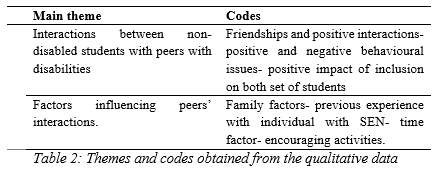
\includegraphics[width=7.5cm]{table 2.png}
    \label{Themes and codes obtained from the qualitative data}
\end{figure}

The fourth stage involved reviewing the themes. During this phase, I made sure that the data within the themes was coherent and that the coded data extracts fitted into the themes. This was achieved by reading and re-reading the entirety of the data to ascertaining whether the themes worked in relation to the data set, as well as to code any additional data that had been missed in earlier coding stages (Braun \& Clarke, 2013). The fifth and final stage of thematic analysis is defining and naming themes. Once these steps were performed, producing the final report was the sixth step, in which the analytic narrative and data extracts are coherently written

\section*{Findings}
Overall, the teachers’ responses indicated that interactions between both student groups are generally positive and teachers believed that this has helped in facilitating the inclusion of students with disabilities. According to 6 out of 8 teachers, non-disabled students accept their peers with disabilities and are making friendships with them. The teachers’ positive responses in this regard were seen in that non-disabled students often helped, made friends and played with peers with disabilities. Many of the interviewed teachers gave positive accounts of how inclusion in mainstream schools and the positive interaction between non-disabled students and students with disabilities have a high impact upon the wellbeing and education experience of the students with disabilities.

 Fostering social relationships in schools and building a supportive school network, which includes other students, was seen as key to promoting inclusion. This was clear from the benefit that the teachers noticed in both groups of students. Evidence regarding this is contained in the following example, where: \textit{“they are not only interacting, but also they learn a lot from each other”} (Teacher 3). Teachers, therefore, were asked in what ways students benefit from the interactions with each other and from inclusion as a whole. Responses on the benefits of inclusion are reported under three main headings: psychological, social, and academic benefits. Psychological benefits identified by special education teachers included developing self-esteem and self-confidence, something which was highlighted by the majority of the interviewed teachers. For example, \textit{"students with disabilities developed a self-esteem and became more confident"} (Teacher 5) which is an opinion reported by all teachers.  
 
The key social benefits identified, however, were the development of social skills and the ability for making friendships, as well as learning through the modelling of appropriate behaviours, as highlighted by the interviewed teachers: \textit{“they used to be quiet and isolated, whereas now almost every student has a friend from general education”} (Teacher 5). This was attributed by the teacher to the activities, such as \textit{“Friends of Students with disabilities Club”} (Teacher 5), which teachers implement in order to get both students with disabilities and non-disabled students to interact. 

The opportunity for social interaction as a part of inclusion was also fundamental, according to interviewees, in improving the speech of students with disabilities. In giving students with disabilities more opportunities to communicate, \textit{“their speech improved a lot”} (Teacher1), and: \textit{“one of the students never talked when she came to the school but now she can say a full coherent sentence”} (Teacher 3). Hence, increased interaction improved both speech and the confidence of students with disabilities. 

 In addition, some academic benefits were also reported by several teachers, for example, \textit{“… their academic performance is gradually improving even though they couldn’t master some skills”} (Teacher 2). A similar response was given by a teacher 5 where she stated : “they are gaining education skills from non-disabled peers and they are making relatively good academic progress”. The benefits of collaboration and interaction were not only noticed for students with disabilities, but also for non-disabled students; \textit{“non-disabled students also improve in their interactions with the students with disabilities through collaboration"} (Teacher 4). Whilst this was the point of view of the majority of the interviewees, negative exceptions were reported by two teachers. Given the above, teachers were then asked what underlying factors that they think contribute to, facilitate, or otherwise obstruct the students’ interactions and relationships. A number of factors were mentioned by the interviewed teachers and are discussed in the following sub-theme.   

\section*{Factors influencing peers’ interactions}
An important factor that teachers think influences the attitudes and interactions of non-\\disabled students towards those with disabilities is that of the surrounding culture and the community. This mainly includes parents, insofar as family plays an important role in enhancing and promoting positive or negative attitudes of their children.  Another factor reported is having previous experience or contact with an individual with disabilities. This was clear when one of the interviewed teachers discussed a case of a student who had a very positive attitude towards students with disabilities in the school, which was seen by the teacher to be based on her experiences at home: one of the students has two deaf brothers and therefore she knows sign language, which she uses with the deaf peers in the school (Teacher 3). Thus, according to the teacher, having prior experience with individuals with disabilities played an important role in forming positive attitudes and acceptance of others with disabilities. From this example, knowing how to communicate with students with disabilities, using sign language in this case, facilitated both students’ interaction. Other teachers, however, believe that this positive interaction comes spontaneously with time and they ultimately accept each other. Some other interviewees believed that the inclusive activities and communities they created and in which both had the opportunity to communicate, were an effective way to foster acceptance and positive interaction.

\section*{Discussion} 
Peers, as social agents, are responsible for the creation of a favourable social environment, in which one of the key factors is a positive and receptive attitude (Reina \& Alvaro-Ruiz, 2016). As stated previously, the participants were overall positive regarding the aspect of non-disabled peers’ interactions with students with disabilities in mainstream schools. This can be explained by the argument presented by the Centre of Studies in Inclusive Education (2008) that, inclusion is the form of education that allows the development of respect, understanding and friendships between non-disabled students and their peers with disabilities. This is because they meet and interact daily and thus learning about each other is an integral part of their education for life. 

The attitudes and behaviour of families of non-disabled children and how that might influence their children’s perceptions and therefore behaviours, either positively or negatively, was one of the main factors reported by the participants in this research.This finding is consistent with previous research by Soodak \& Erwin (2001) who argued that parents’ have a real power in shaping their children’s attitudes towards individual with disabilities, which are vital for the ultimate success of inclusion. In addition, another factor reported is that some students are positive and are interacting with their peers with disabilities more easily because of previous experience or contact with individual with disabilities. This finding corresponds with other previous studies such as McDougall et al., (2004), who discussed how students who have had previously a direct contact with an individual with disabilities, either through their family or a friend, were better able to communicate with them. In such a case, the teacher could take advantage of this situation when attempting to get students working together. For example, a peer tutoring strategy or group activities could be used, in which both non-disabled students and students with disabilities work together and in which such a student could facilitate interaction between the group members (Garrote, 2017). 

Positive interactions between non-disabled students and students with disabilities, as argued by Walker, (2008) requires a supportive environment that encourages meaningful participation of students with disabilities through social interaction with other non-disabled students is important to develop them emotionally and socially.  Teachers in this research reported better efforts made to encourage this positive relationship between students, compared to the previous aspect. According to Mitchell (2014), the role of the teacher is extremely vital to the development of the students as they should be able to create a conducive, comfortable, educative and challenging atmosphere for these students both for the purpose of learning and socialization. The findings of this research confirm those of Mitchell (2014) in that participating teachers in this research reflected an awareness of the importance of their role and believed that the efforts they make to encourage students’ positive interaction is an important factor that facilitates the students’ interactions and acceptance as they have shown noticeable result.

Bruce \& Hansson (2011), argued that positive social interactions among students are essential for the students’ cognitive, social, and language development. The findings of this research further confirmed the argument of Bruce \& Hansson (2011), where teachers also saw the opportunity for social interaction as a part of inclusion as fundamental in improving the speech of students with disabilities, improving their self-esteem and self-confidence as well as learning through the modelling of appropriate behaviours. Such positive behaviours that the students acquired are important and, therefore, should be maintained and encouraged. This is because most of positive social behaviours are of limited use unless they can be shown to generalise to appropriate situations (Pierangelo \& Giuliani, 2008).  According to the social model, the removal of barriers to inclusivity requires a change of approach and thinking in the way how these barriers can be removed (Smith et al., 2014). Therefore, enhancing such positive behaviours and encouraging its generalisation will help in promoting not only inclusive school but also inclusive society. Teachers might do so through using generalisation of positive behaviour by which teachers need to train students to transfer their positive behaviour not only within the school context but also outside the school context. Teachers might ask parents to help in monitoring the students’ generalisation outside the school context by acknowledging positive behaviours of their children, so that they too help in maintaining these behaviours (Pierangelo \& Giuliani, 2008).  

Based on the finding of this research and the previously mentioned studies, it can be suggested that, the positive interactions reported by special education teaches are more likely to be enhanced if general education teachers as well as schools’ head teachers activate their roles and facilitate positive peers’ interactions, thus encouraging both groups of students to understand and accept one another. Through this, a better and more inclusive school culture may be created. A potential means of encouraging schools’ staff to work collaboratively in enhancing students’ positive interactions is by the Local Education Authorities (LEAs) to establish inclusive evaluative criteria for schools, one of which is the extent to which schools’ staff collaborate and participate in planning and conducting activities, encouraging positive interactions of students, as well as working towards enhancing acceptance of all students.

\section*{Conclusion}
Overall, as can be seen from the above, analysing the interviews of special education teachers revealed generally positive findings. It was generally felt that there were very positive effects from inclusion on both non-disabled students and students with disabilities, except some negative findings such as; learning inappropriate words and inappropriate behaviours. Special education teachers reported some efforts in terms of facilitating students’ interactions and friendships, which has shown positive results and has benefitted non-disabled students and students with disabilities alike. Analysis of the interviews also showed that the wider community, and especially parents, have an impact up on how non-disabled students and students with disabilities interacted. It was also felt by the interviewees that various positive reinforcement strategies were helpful. Previous experience with individual with disabilities, time and the availability of shared activities were all reported to be contributing to the enhancement of students’ positive interaction and helped in overcoming initial concerns of ‘difference’. Some interviewees were frustrated by the lack of support from other staff in this aspect and has reported the importance of the role played by head teachers in promoting inclusion of students with disabilities in mainstream schools.

\section*{Acknowledgment}
The authors extend their appreciation to the Deanship of Scientific Research at King Khalid University for funding this work through General Research Project under grant \\number (GRP/259/43).

\include{} 
\section*{References}\par 

\leftskip 0.25in
\parindent -0.25in 
%%%

Al-Darab'h, I., Alrub, M. A., \& Al-Mohtadi, R. M. (2015). What Is the Reality of Preschool in Jordan?. Journal of Education and Practice, 6(10), 180-187

Beacham, N. \& Rouse, M. (2012). Student teachers' attitudes and beliefs about inclusion and inclusive practice. Journal of Research in Special Educational Needs, 12(1), 3-11.‏ \\https://doi.org/10.1111/j.1471-3802.2010.\\01194.x

Bebetsos, E., Derri, V., Filippou, F., Zetou, E., \& Vernadakis, N. (2014). Elementary school children's behavior towards the inclusion of peers with disabilities, in mainstream physical education classes. Procedia-Social and behavioral sciences, 152, 819-823.‏ \\https://doi.org/10.1016/j.sbspro.2014.09.327

Blackburn, C. (2016). Early Childhood Inclusion in the United Kingdom. Infants & Young Children, 29(3), 239-246. \\https://doi.org/10.1097/IYC.00000000000\\00069 

Clarke, V., \& Braun, V. (2013). Successful qualitative research: A practical guide for beginners. Successful Qualitative Research, 1-400.‏

Bruce, B., \& Hansson, K. (2011). Promoting peer interaction. Autism Spectrum Disorders-From Genes to Environment, 23, 313-328.‏ https://doi.org/10.5772/20034

Carter, E. W., Sisco, L. G., Chung, Y. C., \& Stanton-Chapman, T. L. (2010). Peer interactions of students with intellectual disabilities and/or autism: A map of the intervention literature. Research and Practice for Persons with Severe Disabilities, 35(3-4), 63-79.‏ \\https://doi.org/10.2511/rpsd.35.3-4.63

Cole, D. A., \& Meyer, L. H. (1991). Social integration and severe disabilities: A longitudinal analysis of child outcomes. The Journal of Special Education, 25(3), 340-351.‏ https://doi.org/10.1177/002246699102500306 

de Boer, A., Pijl, S. J., Post, W., \& Minnaert, A. (2013). Peer acceptance and friendships of students with disabilities in general education: The role of child, peer, and classroom variables. Social Development, 22(4), 831-844.‏ https://doi.org/10.1111/j.1467-9507.\\2012.00670.x

Diken, I. H., Rakap, S., Diken, O., Tomris, G., \& Celik, S. (2016). Early childhood inclusion in Turkey. Infants & Young Children, 29(3), 231-238.‏ https://doi.org/10.1097/IYC.\\0000000000000065

Dyson, L. L. (2005). Kindergarten children's understanding of and attitudes toward people with disabilities. Topics in Early Childhood Special Education, 25(2), 95-105.‏ \\https://doi.org/10.1177/027112140502500\\20601

Fisher, M., \& Meyer, L. H. (2002). Development and social competence after two years for students enrolled in inclusive and self-contained educational programs. Research and Practice for Persons with Severe Disabilities, 27(3), 165-174.‏ \\https://doi.org/10.2511/rpsd.27.3.165 

Gill, P., Stewart, K., Treasure, E., \& Chadwick, B. (2008). Methods of data collection in qualitative research: interviews and focus groups. British dental journal, 204(6), 291-295.‏ https://doi.org/10.1038/bdj.2008.192 

Jolliffe, W. (2007). Cooperative learning in the classroom: Putting it into practice. Sage.‏ https://doi.org/10.4135/9781446213971 

Guralnick, M. J., Neville, B., Hammond, M. A., \& Connor, R. T. (2007). The friendships of young children with developmental delays: A longitudinal analysis. Journal of Applied Developmental Psychology, 28(1), 64-79.‏ https://doi.org/10.1016/j.appdev.\\2006.10.004 

Harper, C. B., Symon, J. B., \& Frea, W. D. (2008). Recess is time-in: Using peers to improve social skills of children with autism. Journal of autism and developmental disorders, 38(5), 815-826.‏ https://doi.org/10.1007\\/s10803-007-0449-2 

Holahan, A., & Costenbader, V. (2000). A comparison of developmental gains for preschool children with disabilities in inclusive and self-contained classrooms. Topics in Early Childhood Special Education, 20(4), 224-235.‏ https://doi.org/10.1177/027112140002\\000403

Hunt, P., Soto, G., Maier, J., \& Doering, K. (2003). Collaborative teaming to support students at risk and students with severe disabilities in general education classrooms. Exceptional children, 69(3), 315-332.‏ \\https://doi.org/10.1177/001440290306900304 

Kwon, K. A., Elicker, J., \& Kontos, S. (2011). Social IEP objectives, teacher talk, and peer interaction in inclusive and segregated pre\\school settings. Early Childhood Education Journal, 39(4), 267-277.‏ https://doi.org/10.\\1007/s10643-011-0469-6 

Lee, F. L. M., Yeung, A. S., Tracey, D., \& Barker, K. (2015). Inclusion of children with special needs in early childhood education: What teacher characteristics matter. Topics in early childhood special education, 35(2), 79-88.‏ https://doi.org/10.1177/02711214145\\66014

Maras, P., \& Brown, R. (2000). Effects of different forms of school contact on children's attitudes toward disabled and non‐disabled peers. British Journal of Educational Psychology, 70(3), 337-351.‏ https://doi.org/10.\\1348/000709900158164 

McDougall*, J., DeWit, D. J., King, G., Miller, L. T., \& Killip, S. (2004). High School‐Aged Youths' Attitudes Toward their Peers with Disabilities: the role of school and student interpersonal Factors. International Journal of Disability, Development and Education, 51(3), 287-313.‏ https://doi.org/10.1080/\\1034912042000259242 

Mitchell, D. (2014). What really works in special and inclusive education: Using evidence-based teaching strategies. Routledge.‏ \\https://doi.org/10.1080/1034912022000007270 

Nowicki, E. A., \& Sandieson, R. (2002). A meta-analysis of school-age children's attitudes towards persons with physical or intellectual disabilities. International Journal of Disability, Development and Education, 49(3), 243-265.‏

Ogelman, H. G., \& Seçer, Z. (2012). The Effect Inclusive Education Practice during Preschool Has on the Peer Relations and Social Skills of 5-6-Year Olds with Typical Development. International Journal of Special Education, 27(3), 169-175.‏

Peters, S. J. (2004). Inclusive education: An EFA strategy for all children. Washington, DC: World Bank, Human Development Network.‏

Pierangelo, R., \& Giuliani, G. (2008). Teaching students with learning disabilities: A step-by-step guide for educators. Corwin Press.‏

Reina, R., \& Alvaro-Ruiz, J. (2016). Full inclusion of a student with visual impairment over the full Physical Activity and Sport Sciences Degree: A case study. European Journal of Adapted Physical Activity, 9(1).‏ https://doi.org/10.5507/euj.2016.004\\ https://doi.org/10.5507/euj.2016.004

Qu, S. Q., \& Dumay, J. (2011). The qualitative research interview. Qualitative research in accounting \& management.‏ 

Smith, T. E., Polloway, E. A., Patton, J. R., Dowdy, C. A., \& Doughty, T. T. (2014). Teaching students with special needs in inclusive settings (Vol. 6). Upper Saddle River, NJ: Pearson.‏

Soodak, L. C., \& Erwin, E. J. (2000). Valued member or tolerated participant: Parents' experiences in inclusive early childhood settings. Journal of the Association for persons with severe handicaps, 25(1), 29-41.‏ https://doi.org/10.2511/rpsd.25.1.29 

Thomas, G. (2017). How to do your research project: A guide for students. Sage.‏

Walker, S., \& Berthelsen, D. (2008). Children with autistic spectrum disorder in early childhood education programs: A social constructivist perspective on inclusion. International Journal of Early Childhood, 40(1), 33-51.‏ https://doi.org/10.1007/BF03168362 


\include{} 


\endleftskipleftskip 
\endparindentparindentparindentparindent

\newpage

\section*{Appendix A: Interview}\par 

Participant perceptions about memorable activities during the summer DES session. 


\begin{figure}[htp]
    \centering
    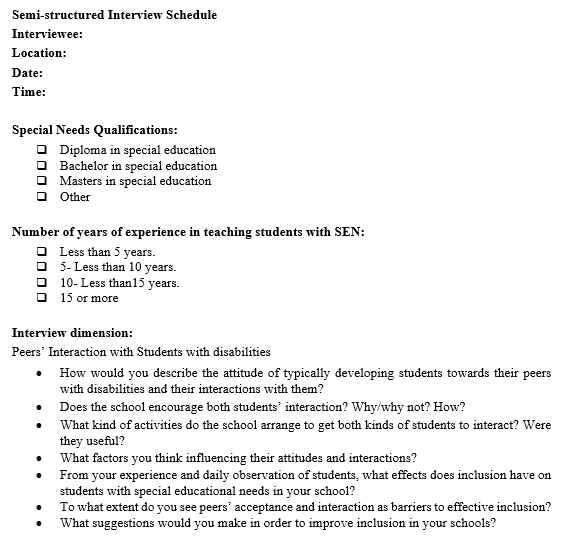
\includegraphics[width=8cm]{appendix a.png}

\end{figure}


\end{large}
\end{document}
